\documentclass[a4paper]{article}

\usepackage[english]{babel}
\usepackage{amsmath}
\usepackage{float}
\usepackage{amssymb}
\usepackage{dsfont}
\usepackage{graphicx}
\usepackage{listings}
\usepackage[hyphens]{url}
\usepackage{titling}
\usepackage{varwidth}
\usepackage{hyperref}
\usepackage{url}
\usepackage{adjustbox}
\usepackage{color} %red, green, blue, yellow, cyan, magenta, black, white
\definecolor{mygreen}{RGB}{28,172,0} % color values Red, Green, Blue
\definecolor{mylilas}{RGB}{170,55,241}


\usepackage{geometry}
 \geometry{
 a4paper,
 total={165mm,257mm},
 left=20mm,
 top=20mm,
 }

\title{Natural Computing\\Assignment 4}
\author{
  Christoph Schmidl\\ s4226887\\      \texttt{c.schmidl@student.ru.nl}
  \and
  Koen Vijverberg\\ s4132858\\     \texttt{koen.vijverberg@student.ru.nl}
  \and
  Alex Kolmus\\	s4125304\\	\texttt{alex.kolmus@student.ru.nl}
}
\date{\today}

\begin{document}
\maketitle


\subsection*{Evolutionary Game Theory and Cellular Automata}

\begin{enumerate}

	% Task 1	
	\item(Nash equilibria and ESS's.) Find Nash equilibria and ESS's for each of the following payoff matrices.
	
	\begin{enumerate}
		% Task 1a	
		\item 
		\begin{minipage}[t]{\linewidth}
          \centering
          \adjustbox{valign=t}{%
            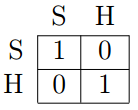
\includegraphics[width=.15\linewidth]{./images/task1a.PNG}%
          }
    \end{minipage}
    \vspace{1em}
		\textbf{Solution:}\\
		
		\textbf{Definition "ESS":} A pure ESS is a strategy that cannot be invaded by another strategy.\\
		
		If all population members are S or H respectively, then all get a payoff of 1. If an H mutant appears in a population of all S then both get a payoff of 0 and vice versa. Both S and H are ESSs, because neither can be invaded by the other. The strategy that dominates over time is the one that starts in the majority.
		\vspace{1em}
		
		\textbf{Definition "Strict Nash Equilibrium":} A pair of strategies is a strict Nash equilibrium if neither player can unilaterally switch to another strategy without reducing its payoff.\vspace{1em}
		
		The upper-left cell (S,S) is a strict Nash equilibrium. Possible switches are as follows: (S,H) and (H,S). Both switches reduce the payoff of 1 to 0 which makes it a nash equilibrium.\\
		
		The bottom-right cell (H,H) is a strict Nash equilibrium. Possible switches are as follows: (S,H) and (H,S). Both switches reduce the payoff of 1 to 0 which makes it a nash equilibrium.
		\vspace{1em}
		
		
		% Task 1b	
		\item \begin{minipage}[t]{\linewidth}
          \centering
          \adjustbox{valign=t}{%
            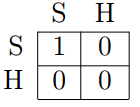
\includegraphics[width=.15\linewidth]{./images/task1b.PNG}%
          }
    \end{minipage}
    \vspace{1em}
		\textbf{Solution:}\\
		
		\textbf{ESS}\\
		
		If all population members are S , then all get a payoff of 1.\\
		If all population members are H , then all get a payoff of 0. S is a ESS, because it cannot be invaded by any other strategy.\\
		
		
		\textbf{Nash Equilibrium}\\
		
				The upper-left cell (S,S) is a strict Nash equilibrium. Possible switches are as follows: (S,H) and (H,S). Both switches reduce the payoff of 1 to 0 which makes it a nash equilibrium.\\
		
		
		
		
		% Task 1c
		\item \begin{minipage}[t]{\linewidth}
          \centering
          \adjustbox{valign=t}{%
            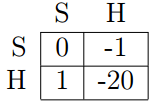
\includegraphics[width=.15\linewidth]{./images/task1c.PNG}%
          }
    \end{minipage}
    \vspace{1em}		
        \textbf{Solution:}\\
        
        
	    There are two pure strategy Nash equilibria in this game (H,S) and (S,H). However, in the absence of an uncorrelated asymmetry, neither H nor S are Esses. There is a third Nash equilibrium which represents a mixed strategy and is also an ESS. A mixed strategy is a strategy in which a player plays his available pure strategies with certain probabilities.\\
	    
	    \begin{itemize}
	        \item Expected payoff of S $p(0) + (1 - p)((-1))$
	        \item Exceptected payoff of H is $p(1) + (1 - p)(-20)$
	        \item The two types do equally well when $p(0) + (1 - p)((-1)) = p(1) + (1 - p)(-20)$
	    \end{itemize}
	    
\begin{align*}
    p(0) + (1 - p)((-1)) &= p(1) + (1 - p)(-20)\\
    -1 - p &= p - 20 + 20p\\
    -20p &= 21\\
    p &= -\frac{21}{20}
\end{align*}
		
		% Task 1d	
		\item Interpret the results of the previous exercises. What can you say about Nash equilibria, ESS's and their relation?\\
		\textbf{Solution:}\\	
		
		Nash equilibria are defined on strategy sets (a specification of a strategy for each player or population), while ESS are defined in terms of strategies themselves. As we see in the last task, an ESS is also a Nash equilibrium but this assumption does not hold the other way around, therefore an Nash equilibrium does not need to be an ESS.\vspace{1em}
		
		
		
		
		
	\end{enumerate}
	
	% Task 2
	\item(Replicator Dynamics.) Consider the pairwise contest with actions A and B and payoff matrix.
	
		\begin{figure}[H]
	    \centering
  	    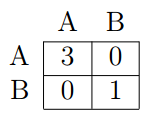
\includegraphics[width=0.15\textwidth]{images/task2.PNG}
	    \end{figure}	
	
	
	\begin{enumerate}
		% Task 2a
		\item What are the Ess of this game?\\
		\textbf{Solution:}\\
		
		A is ESS if
		
		\begin{enumerate}
		    \item[a] $P(A,A) \geq P(B,A)$
		    \item[b] Moreover if $P(A,A) = P(B,A)$ then $P(A,B) > P(B,B)$
		\end{enumerate}
		
		Therefore, A is an ESS.\\
		
		B is ESS if
		
		\begin{enumerate}
		    \item[a] $P(B,B) \geq P(A,B)$
		    \item[b] Moreover if $P(B,B) = P(A,B)$ then $P(B,A) > P(A,A)$
		\end{enumerate}
		
		Therefore, B is no ESS.\\
		
		
		
		
		% Task 2b
		\item Denote by $x$ the fraction of the population using A.
			\begin{enumerate}
				% Task 2b i.
				\item Compute the expected payoff of (a player with) strategy A, of strategy B, and the total expected payoff of a player.\\
				\textbf{Solution:}\\
				
				\textbf{Definition: "Expected payoff of a strategy":} Suppose a strategy $s$ is played against strategies S1, ..., Sn. Then the expected payoff of s is the sum of the payoffs of s against each of the $S_i$ times the probability that $S_i$ is played.\\
				
                \textbf{Definition: "Average expected payoff of a population"} is the expected payoff of S1 times the probability that S1 is played plus the expected payoff of S2 times the probability that S2 is played plus ... the expected payoff of Sn times the probability that Sn is played.\\
				
				
				
								This exercise represents a game with strategies A,B and the following payoffs:
				
												\begin{align*}
				    \pi(A,A) = 3, \pi(A,B) = 0, \pi(B,A) = 0, \pi(B,B) = 1
				\end{align*}
				\vspace{1em}
				
				
				The total expected payoff of a player is therefore:
				
				\begin{align*}
				    \pi(A,x) = 3x_1 + 0(1 - x_2) &= 3x_1 \quad \text{and} \quad \pi(B,x) = 0x_1 + 1(1-x_2) = 1 - x_2\\
				    &= \bar{\pi}(x) = x_1(3x_1) + x_2(1 - x_2)\\
				    &= 3x_1^2 + x_2 - x_2^2
				\end{align*}
				
				
				
				% Task 2b ii.
				\item Give the replicator dynamics equation for this game.\\
				\textbf{Solution:}\\
				

				
				\begin{align*}
				    \dot{x} = x(1 - x)(\pi(S_1, x) - \pi(S_2, x))
				\end{align*}
				
				Then 
				
				\begin{align*}
				    \pi(A,x) = 3x + 0(1 - x) = 3x \qquad ; \qquad \pi(B,x) = 0x + 1(1 - x) = 1 - x
				\end{align*}
				

                \begin{align*}
                    \dot{x} &= x(1-x)(\pi(A,x) - \pi(B,x))\\
                    &= x(1-x)(3x - (1 - x))\\
                    &= x(1-x)(4x - 1)
                \end{align*}
				
				
				
				
				% Task 2b iii.
				\item Find the fixed points.\\
				\textbf{Solution:}\\
				
				\textbf{Definition "Fixed point":} A fixed point of the replicator dynamics is a population that satisfies $\dot{x}_i = 0 \forall i$. Fixed points describe populations that are no longer evolving, that is, there is no change of strategies in time.\vspace{1em}
				
				Fixed points are:
				
				\begin{align*}
                    \dot{x} &= x(1-x)(4x - 1) = 0\\
                    x &= 0,  1 - x = 0, 4x -1 = 0\\
                    x &= 0, x = 1, x = \frac{1}{4}
                \end{align*}
				
				all of them are between zero and one, so they represent legitemate fractions.
				% Task 2b iv.
				\item Which fixed points are evolutionary end points? (Motivate your answer)\\
				\textbf{Solution:}\\
				We have to determine the derivative around the fixed points, if they are stable fixed points (a point in the neighbourhood will converge towards it) they are evolutionary end points. (We just want to find the derivative around the point).
				
				\begin{align}
				    \dot{x}(x = 0.01) = - 0.009
				\end{align}
				
				
				\begin{align}
				    \dot{x}(x = 0.24) = -0.007
				\end{align}
				
				\begin{align}
				    \dot{x}(x = 0.26) = 0.007
				\end{align}
				
				\begin{align}
				    \dot{x}(x = 0.99) = 0.03
				\end{align}
				
				So the fixed point at $x=0.25$ is unstable(points around 0.25 move away from it), which automatically means that $x=0$ and $x=1$ are stable (but we checked anyways ...). Which results in $x = 0, 1$ being the two evolutionary end points.
				
			\end{enumerate}
	\end{enumerate}	
	
	
	% Task 3
	\item (Experimenting with existing software.) Consider the NetLogo model available at\\ \url{http://ccl.northwestern.edu/netlogo/models/community/GameTheory}	
	
	\begin{enumerate}
		% Task 3a
		\item Run the model following the steps described in the \texttt{\#\# HOW TO USE IT} section. Try to justify the results obtained using the different setting described in the section.\\
		\textbf{Solution:}\\
		
		Run the model with only doves and hawks. Start with equal numbers of each type, and with the value of the resource greater than twice the cost of fighting. The doves will go extinct.

\textit{Indeed the doves go extinct, if the value is set to 5 en the cost to 2. The doves go extinct, this can be understood if we take a look at the following payoff matrix:}

\begin{table}[h]
    \begin{center}
    	\begin{tabular}{lll}
    			 & hawk     & dove    \\
    		hawk & 1.5,1.5, & 5,0     \\
    		dove & 0,5      & 2.5,2.5
    	\end{tabular}
	\end{center}
\end{table}

\textit{The Hawk option is simply the most profitable option. Since it will always get it is resources faster (on average) then the dove.}

Now try the same again, but have the value of resource greater than the cost, but less than twice as great. A stable polymorphism should result.

\textit{Indeed a stable polymorphism arises, the hawk - dove ratio/equilibrium is 3:1 for value = 3 and cost = 2. This equilibrium can be understood in the following way, for the 3:1 ratio the grow rate is equal! The hawk and dove get the following value:}
\begin{table}[h]
    \begin{center}
    	\begin{tabular}{lll}
    			 & hawk     & dove    \\
    		hawk & 0.5,0.5, & 3,0     \\
    		dove & 0,3      & 1.5,1.5
    	\end{tabular}
    \end{center}
\end{table}
\begin{align}
	Profit_{Hawk} &= 0.5*P(H, H) + 3*P(H, D) = 0.5*3/4 + 3*1/4 = 9/8\\
	Profit_{Dove} &= 1.5*P(D, D) = 1.5*1.5 = 9/8
\end{align}

Next, set the cost of fighting greater than the value of the resource. The polymorphism is still stable, but the level has changed.

\textit{If we set the cost to 3 and the value to 2, the hawk - dove ratio/equilibrium becomes 1:2. Following the same logic as the previous question (the expected value is the same for the dove and hawk).}

\begin{table}[h]
    \begin{center}
    	\begin{tabular}{lll}
    			 & hawk       & dove    \\
    		hawk & -0.5,-0.5, & 2,0     \\
    		dove & 0,2        & 1,1
    	\end{tabular}
	\end{center}
\end{table}

Finally, put some retaliators in the population, set v > 2c and run again. Now, there is an unstable polymorphism. Try different runs with the same settings. Vary the initial numbers of each type of organism.

\textit{Two scenarios seem to exist. The first the hawks drive the doves to extinction. Then the hawks go extinct (since the retaliators will always have a better expectation value then the hawks). The second scenario the Hawks die first and immediately the dove and retaliator plateau due to them having the same expectation value.} 
		
		% Task 3b
		\item Discuss briefly your experience with the use of such software (pro's and con's).\\
		\textbf{Solution:}\\
		
		In hindsight it was pretty user friendly and not too complicated (there was the initial 2 minutes of confusion with the program/downloading, but that is to be expected). However it remains a black box, if I would like to access the code and understand what is happening exactly I cant (or at least it is difficult to access). Due to the intuitive results and theoretical explanation I trust that it works properly. Furthermore changing the inner workings is only possible by changing the few sliding bars available, any larger changes (creating an extra variable, e.g. disease spreading) is not possible.
		
		
	\end{enumerate}		
	
	% Task 4
	\item Consider the following sequence of states from a 1-D CA:\\
	Use the format in the scheme below (that is, specify the row 'New') to describe two sets of rules able to generate this sequence of states.
	
		\begin{figure}[H]
	    \centering
  	    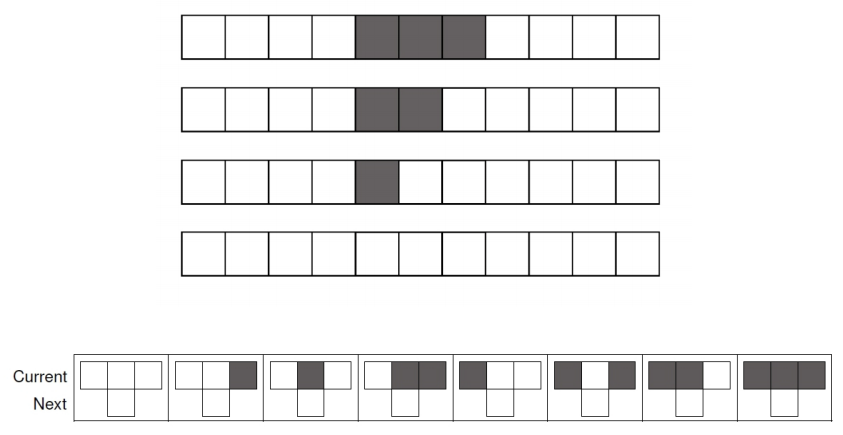
\includegraphics[width=0.7\textwidth]{images/task4.PNG}
	    \end{figure}	
	
	
	
	\textbf{Solution:}\\
	
	\begin{figure}[H]
	    \centering
  	    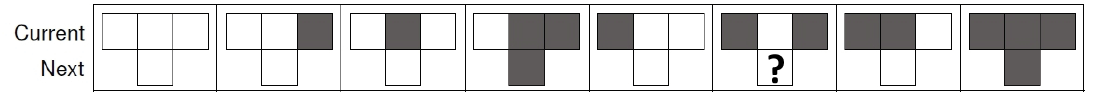
\includegraphics[width=0.7\textwidth]{images/CA_1D.png}
	\end{figure}
	
	The above picture describes the two sets of rules. Since the question mark is not relevant for generating the sequence above it can be black or white, so two different sets of rules in 1 picture.
	
	% Task 5
	\item Download and run the Game of Life simulator from \url{https://bitstorm.org/gameoflife/} Select "Small Exploder" from the menu, click start and wait until a stable state is eached. Explain why this state remains static.\\
	\textbf{Solution:}\\\\
	The static state looks like this:
	\begin{figure}[H]
	\centering
  	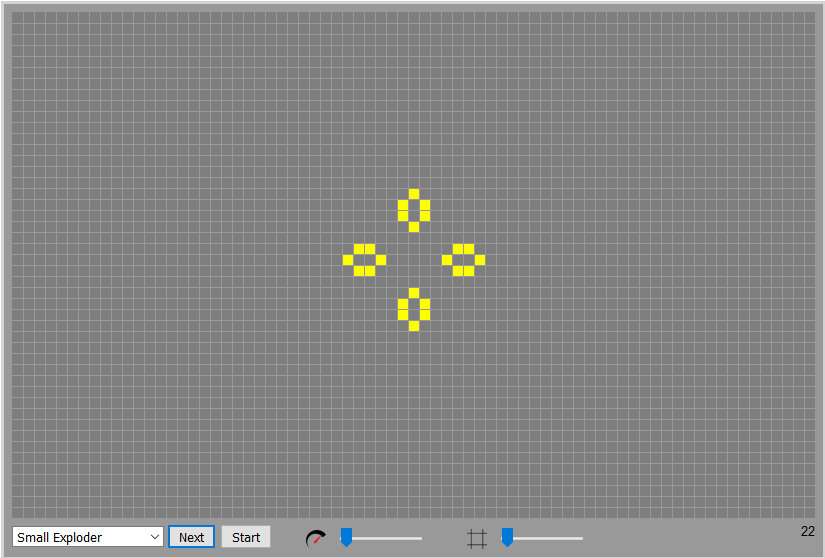
\includegraphics[width=0.7\textwidth]{images/ex_5_small_exploder.png}
	\end{figure}
	
	These structures are identical except for their orientation, we will reason about one of them, which translates to all others. The game of life has the following rules:
	\begin{itemize}
	    \item If a node is alive, and has two or three alive neighbours it stays alive
	    \item If a node is dead, it becomes alive if it has exactly three living neighbours.
	\end{itemize}
	
	We see the following properties in one of the observed static structures:
	\begin{itemize}
	    \item The two dead cells inside have five neighbours each, thus remain dead.
	    \item The alive cells each have two neighbours, thus remain alive.
	    \item The cells around the structure have a maximum of two connected living cells, thus remain dead.
	\end{itemize}
	These properties combined result in the structure remaining in a stable/static state.
	
\end{enumerate}
\end{document}